%This part of the report is to be merged in overleaf with the others, the packages needed are used in the merged TeamF-report.tex document
\begin{document}

\section{Methods}\label{sec:Methods}
In order to create histograms, showing when the warmest and coldest days typically occurred from $1722$ up to $2013$ in Uppsala, two
arrays respectively storing the hottest and coldest day for each year are needed. The code \texttt{Sara{\_}Producefiles.cpp} was written in order to read the data of
the SMHI recorded from Uppsala and then produce two output files:
\begin{itemize}
\item one file called \texttt{year\_hotday\_coldday.dat}, containing a list of the years with the corresponding hottest and coldest days; 
\item a second file called \texttt{years\_days\_temps.dat}, containing most of the recorded temperatures (the criterion for the exclusion of some temperatures is explained below) with the corresponding day 
(from 1 to 366) and year.
\end{itemize}
\medskip
Since not all the data contained in the file from the SMHI were  recorded from the same place, all the readings from a region other
than Uppsala should be ignored. In the first output file the code returns $0$  for the years in which no temperature was measured in Uppsala (and also for the corresponding hottest and coldest days). In the second output file a line of "$0$" is present for each temperature not recorded in the region of interest.

\medskip
\medskip
The data from the Uppsala.dat file are read into a two-dimensional array. The functions \texttt{Function{\_}max} and \texttt{Function{\_}min} are used inside a loop over the first column of the array (containing all the years associated to the temperatures recorded in the 
SMHI file) in order to find the hottest temperature and the coldest temperature of each year with the associated days. The maximization
and minimization are achieved by comparing each temperature with the one stored in the following line, so that the higher/lower temperature between the two is written over the one previously stored in the variable \texttt{Tmax\_temporary} or \texttt{Tmin\_temporary}. The two functions store temperature and day in an array and return the pointer to the array. The function \texttt{NumberoutofDate}
is used in the two functions mentioned above and, if the two-dimensional array and the line of the hottest/coldest temperature
are passed, it returns a number between 1 and 366 corresponding to the day in which that specific temperature has been recorded. 

\medskip

The loop cycle in which the functions mentioned above are called produces an array containing a list of the years, and two arrays containing the hottest and coldest days respectively. These three arrays are printed in the first output file of the code.
The arrays needed to produce the second output file are generated in the second loop of the code.

\medskip
\medskip

A ROOT macro \texttt{Sara{\_}Analyze.C}  was then written in order to read the files produced by the first code and store the data of each column in a different array, but excluding the lines containing $0$ in the first column. An array is produced by the macro for each column of the two files and the so obtained arrays are exploited for producing graphs and histograms.

\medskip
\medskip
Two overlaying histograms are produced by calling the class \texttt{TH1} : one for the distribution of the hottest days and one showing the distribution of the coldest days. The histogram for the hottest days is fitted with a Gaussian function and the mean of the distribution is returned with its uncertainty in order to predict when the hottest day is more likely to occur. The second histogram is fitted with two Gaussian functions since the coldest days mainly occur both at the end of the year and at the beginning. The hottest and coldest days are
plotted either against the years in which thy occur in two separate graphs, by calling the class \texttt{TGraph}.

\medskip
\medskip

The \texttt{2DGraph} class in ROOT is used to obtain two different views of the three-dimensional graph showing how the temperatures in Uppsala changed over the days of the years from 1722 to 2013.The option \texttt{Draw("surf1")} is used to obtain a graph as the one showed in fig.\ref{fig:3D}. The option \texttt{Draw("colz")} is used to obtain a view from the top of the graph.


\section{Results}\label{sec:Results}

The overlaying histograms showing the distribution of the hottest and the coldest days are shown in figure \ref{fig:HotColdHist}.
The mean obtained for the distribution of the hottest days is $193 \pm 2$. The graphs showing how the hottest days and coldest days changed over the years are shown in figures  \ref{fig:HotGraph} and \ref{fig:ColdGraph}. 


\begin{figure}[H]
\begin{center}
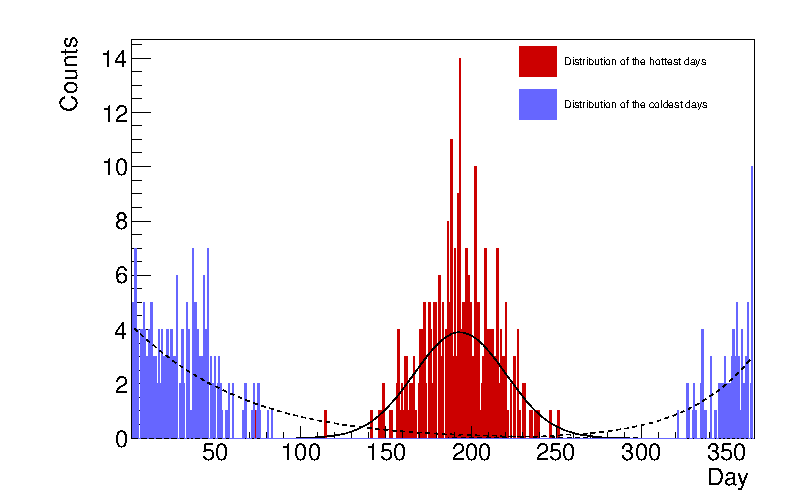
\includegraphics[width=0.9\textwidth]{HottestColdest.png}
\caption{Histogram showing how often each day of the year was the warmest or coldest from 1722 to 2013. Lines show Gaussian fits of the two distributions.}
\label{fig:HotColdHist}
\end{center}
\end{figure}

\begin{figure}[H]
\begin{center}
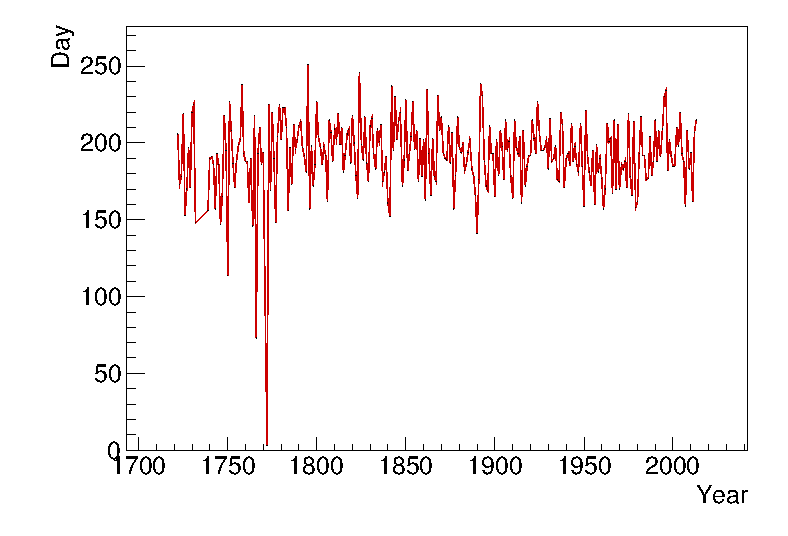
\includegraphics[width=13cm]{graph1DHot.png}
\caption{Graph showing the hottest day for each year from 1722 to 2013.}
\label{fig:HotGraph}
\end{center}
\end{figure}

\begin{figure}[H]
\begin{center}
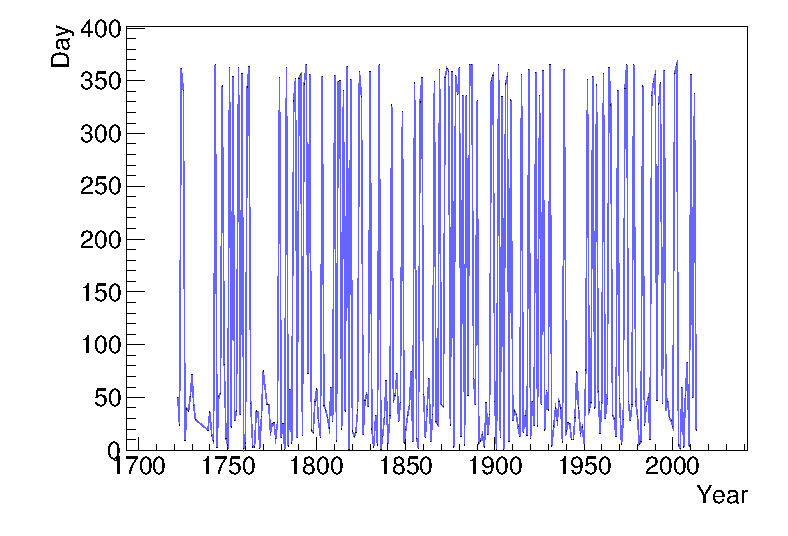
\includegraphics[width=11cm]{graph1D.png}
\caption{Graph showing the coldest day for each year from 1722 to 2013.}
\label{fig:ColdGraph}
\end{center}
\end{figure}

\begin{figure}[H]
\begin{center}
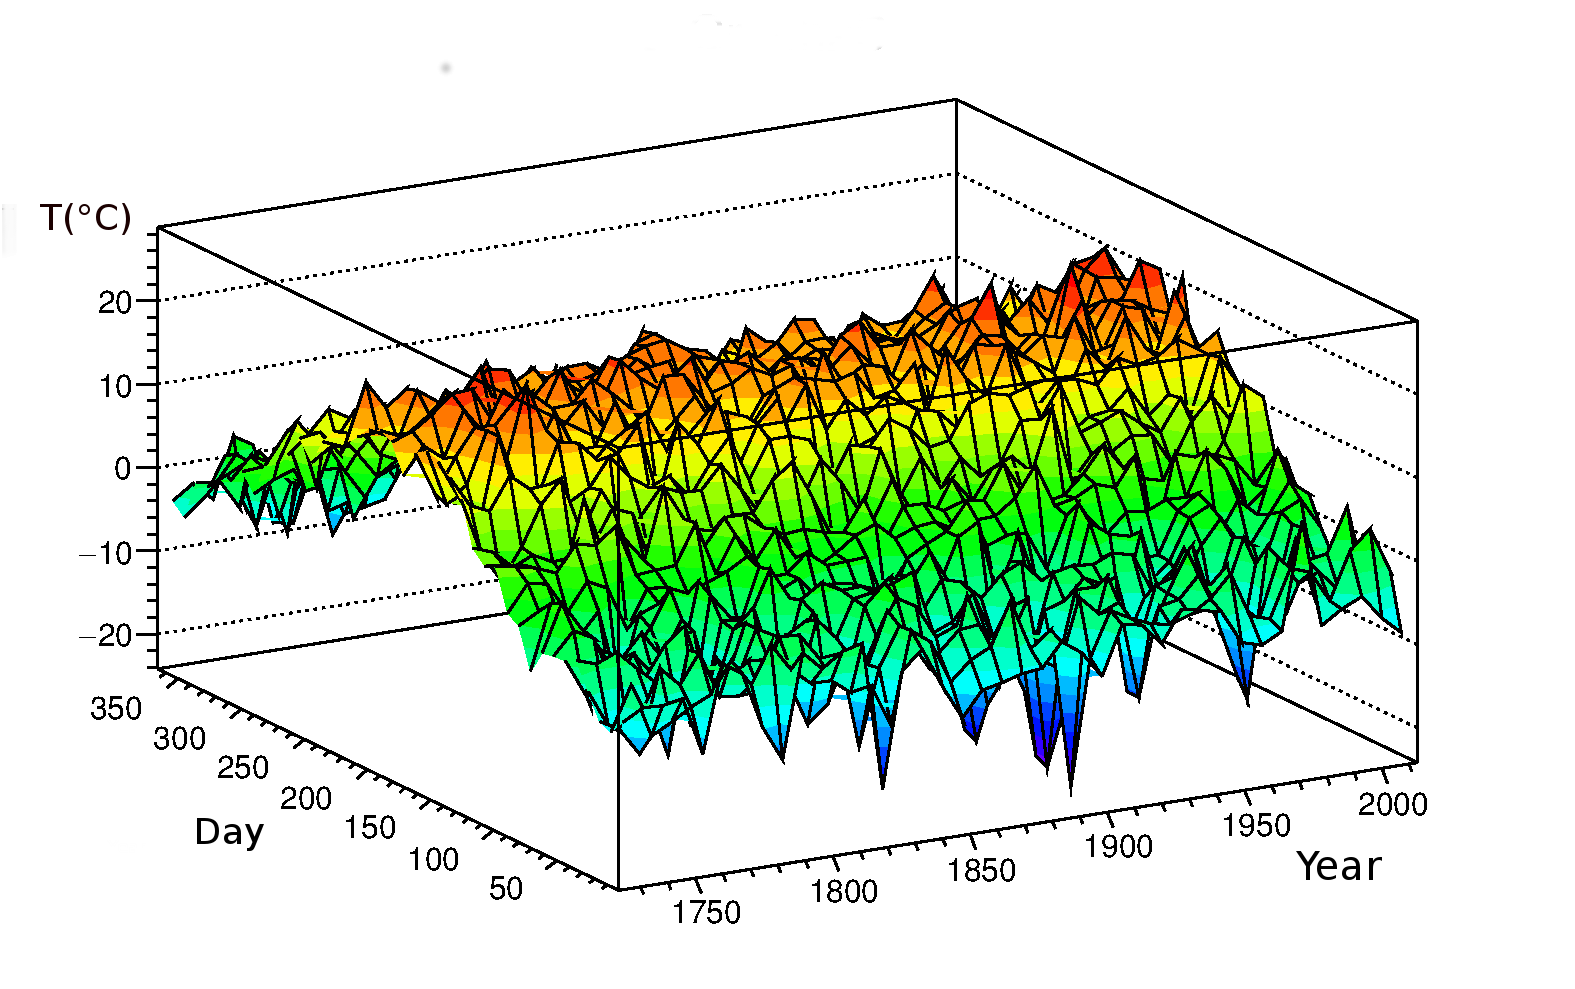
\includegraphics[width=0.9\textwidth]{2Dgraph1.png}
\caption{Graph showing how the temperatures in Uppsala changed over the days of the years from 1722 to 2013.}
\label{fig:3D}
\end{center}
\end{figure}

\begin{figure}[H]
\begin{center}
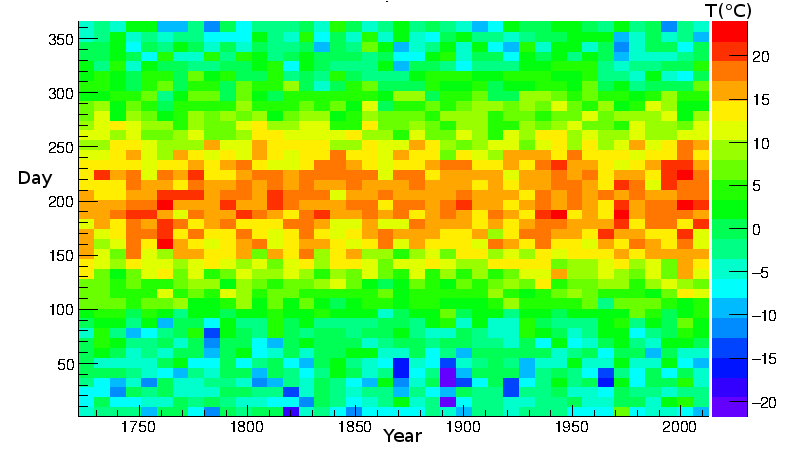
\includegraphics[width=11cm]{2Dgraphint.png}
\caption{View from the top of the Graph in figure \ref{fig:3D}.}
\label{fig:top3D}
\end{center}
\end{figure}


\section{Discussion}\label{sec:Discussion}
Figure \ref{fig:HotColdHist} shows that the hottest temperature in Uppsala is most likely to be registered around the day $193$ (corresponding to July 12 on a regular year). Despite the fitting with Gaussian functions, it is not possible to determine an average of the distribution of the coldest days since it is split into two parts at the beginning and at the end of the year. Consequently another histogram, which is shown in figure \ref{fig:HotColdHist2}, has been obtained where the left part of the histogram (from day 1 to 99) is shifted to the right ( so that the days from 1 to 99 in the first histogram in figure \ref{fig:HotColdHist} correspond to the days from 376 to 465 in figure \ref{fig:HotColdHist2}). In this way we can notice that the mean of the Gaussian function fitting the histogram of the coldest days in figure \ref{fig:HotColdHist2} is 383, and thus the coldest temperature is most likely to be measured in the day number 17 (January 17) with an uncertainty of 3 days.

\begin{figure}[H]
\begin{center}
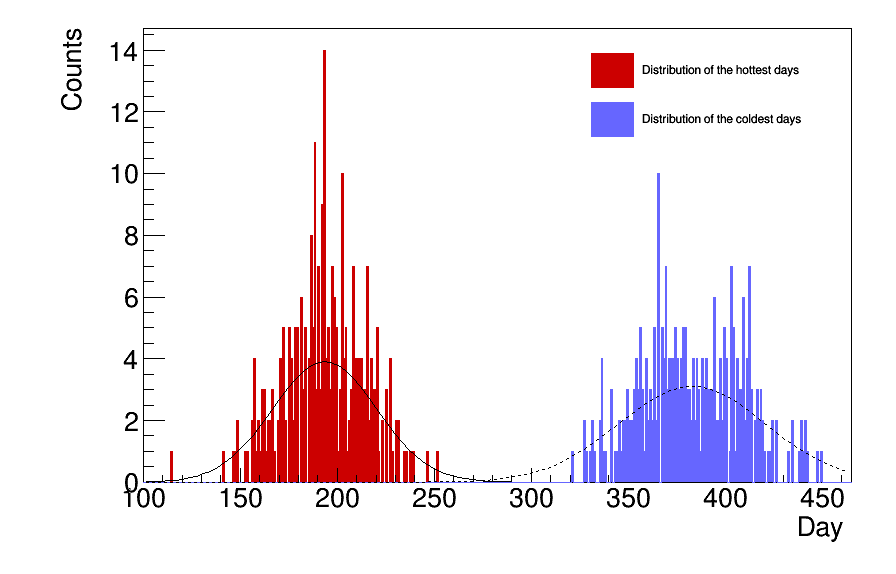
\includegraphics[width=0.7\textwidth]{HotCold_shifted.png}
\caption{"Shifted histogram" obtained by moving the left part of figure \ref{fig:HotColdHist} to the right.}
\label{fig:HotColdHist2}
\end{center}
\end{figure}


Figures \ref{fig:HotColdHist} and \ref{fig:HotGraph} besides show some unexpected values for the hottest days. This is due to the exclusion of some temperatures as described in section
\ref{sec:Saras method}. For some of the years most (and sometimes all) of the temperatures were recorded from regions
different from Uppsala and this implies that for those years less days were candidate for being the hottest or the coldest. 

\medskip
\medskip
The aim of the three-dimensional graph was to point out eventual modifications in the seasonal change, for example a shift in the start of summer. However, none of these changes were observed and apparently the effect of global warming is not evident either. This result might appear contradictory to what we obtained in figure \ref{global_warming_figure}, but this is maybe due to two factors:
\begin{itemize}
\item a change of about $2 \hspace{1mm} ^\circ C$ is not observable in the color coding used for the temperature in figure \ref{fig:top3D};
\item while in figure \ref{global_warming_figure} average temperatures are considered for each year, in the three-dimensional graphs all the daily temperatures are considered.
\end{itemize}

 
 \end{document}
